\documentclass[10pt]{article}
\usepackage{amsmath,textcomp,amssymb,geometry,graphicx,enumerate,tikz,algorithm,algpseudocode,pifont,upgreek}
\usetikzlibrary{calc}
\usetikzlibrary{datavisualization}
\usetikzlibrary{datavisualization.formats.functions}


\textheight=9in
\textwidth=7in
\topmargin=-.75in
\oddsidemargin=-0.25in
\evensidemargin=-0.25in

\usepackage{listings}
\lstnewenvironment{codeblock}
    {\lstset{language=Python,
      showspaces=false,
      showtabs=false,
      breaklines=true,
      mathescape=true,
      showstringspaces=false,
      breakatwhitespace=true,
      commentstyle=\textit,
      keywordstyle=\textbf,
      basicstyle=\ttfamily,
      escapechar=`,
      moredelim={**[is][{\color{RoyalBlue}}]{\^^M\\beginsol}{\^^M\\endsol}},
      moredelim={[is][{\color{RoyalBlue}}]{\^^M\\beginexp}{\^^M\\endexp}},
    }}
    {}

\newcommand{\bigo}{\mathcal{O}}


\begin{document}
\section*{04/06/2016}
\subsubsection*{Heuristic for Avoiding Bad Local Minima (continued)}
\begin{itemize}
	\item Train several nets; pick best. 
	\item \underline{Layer-wise pre-training}
\end{itemize}

\subsection*{Heuristics for Faster Training}
\begin{itemize}
	\item 1, 2, 3, 4 from last lecture.
	\item Stochastic gradient descent faster than batch gradient descent on large, redundant data sets. One \underline{epoch} presents every training example once. Training usually takes many epochs, but if data is huge it can take less than one.
	\item \underline{Normalizing} the data:
		\begin{enumerate}
			\item \underline{Center} each feature so mean is zero (gets sigmoid into good operating region).
			\item Then scale each feature so variance is constant ($\sim 1$ is good). This makes objective function well conditioned. Condition number of a matrix is the largest eigenvalue divided by smallest eigenvalue gives a measure of how acentric the ellipsoids are which gives an idea how much time we'll spend zig-zagging before getting to the minimum.
		\end{enumerate}
	\item Normalizing data:
		\begin{center}
			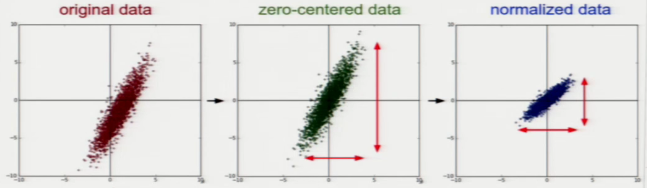
\includegraphics[scale=0.7]{../images/centereddata}
		\end{center}
	\item Centering the hidden units helps too.
		\begin{enumerate}
			\item Replace sigmoids with $2s(\gamma) - 1$ or with $\tanh \gamma$.
		\end{enumerate}
	\item Use different learning rate for each layer of weights. Gradients are much smaller for early layers than later layers.
		\begin{center}
			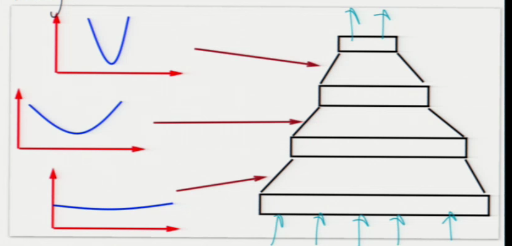
\includegraphics[scale=0.6]{../images/layerdifference}
		\end{center}
	\item \underline{Emphasizing schemes}:
		\begin{itemize}
			\item Shuffle so successive examples are never/rarely same class.
			\item Present examples from rare classes more often, or with bigger learning rate $\epsilon$.
			\item Warning: can backfire on bad outliers.
		\end{itemize}
	\item Second-order optimization.
		\begin{itemize}
			\item No Newton's method: Hessian too expensive.
			\item Nonlinear conjugate gradient; for small nets + small data + regression. Batch descent only! $\rightarrow$ too slow with redundant data.
			\item Stochastic Levernberg Marquardt; approximates a diagonal Hessian.
		\end{itemize}
\end{itemize}

\subsection*{Heuristic to Avoid Overfitting}
\begin{itemize}
	\item Ensemble of neural nets. Random weights; bagging. Slow!
	\item $L_{2}$ regularization, aka \underline{weight decay}. Add $\lambda ||w||^{2}$ to the cost/loss function, where $w$ is vector of all weights. Effect: $\frac{\partial J}{\partial w_{i}}$ has extra term $-2\lambda w_{i}$. Weight decays by factor $(1-2\lambda)$ if reinforced by training.
		\begin{center}
			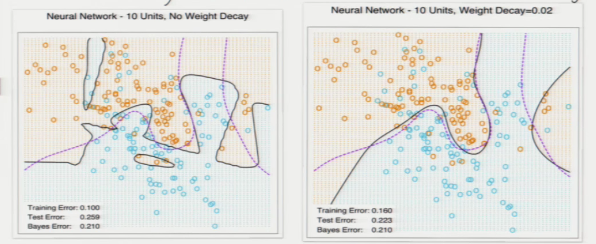
\includegraphics[scale=0.6]{../images/weightdecay}
		\end{center}
	\item \underline{Dropout} emulates an ensemble in one network. (Faster training too).
\end{itemize}

\subsection*{Convolutional Neural Networks (ConvNets)}
\begin{itemize}
	\item Vision: inputs are large images. 200x200 = 40,000 pixels.
	\item If we connect them all to 40,000 hidden units $\rightarrow$ 1.6 billion connections.
	\item Neural nets are often \underline{over-parametized}: too many weights, too little data.
	\item ConvNet ideas:
		\begin{enumerate}
			\item Local connectivity: A hidden unit (in early layer) connects only to small patch of units in previous layer.
			\item Shared weights:
				\begin{itemize}
					\item Groups of hidden units share same set of input weights, called a \underline{mask/filter/kernel}.
					\item We learn several masks.
					\item Masks x patches = hiddent unit (in first hidden layer).
					\item If one patch learns to detect edges, every patch has an edge detector.
					\item ConvNets exploit repeated structure in images, audio.
					\item \underline{Convolutions}: the same linear transformation applied to different parts of image by shifting.				
				\end{itemize}
		\end{enumerate}
\end{itemize}
\end{document}